\begin{center}
	\section{CFD-DEM}
\end{center}

\noindent
\justify

En el acoplamiento cl\'asico entre CFD-DEM, el flujo se resuelve a trav\'e del m\'etodo CFD basado en malla, mientras que la fase s\'olida es modelada mediante DEM para cada part\'icula sujeta a trav\'es de fuerzas hidrodin\'amicas, fuerzas de cuerpo (como la gravedad) y a trav\'es de fuerzas de contacto, actualizando valores de velocidad y posici\'on conforme a la segunda ley de Newton (Hoomans \textit{et al.}, 1996; Tsuji \textit{et al.}, 1993; Xu y Yu, 1997). En principio, todos los m\'etodos CFD pueden acoplarse con DEM; lo que ha dado origen a diferentes m\'etodos discretos y continuos, tal como el m\'etodo de Lattice Boltzmann (LBM), Hidrodin\'amica de Part\'iculas Suaves (SPH), m\'etodos de Diferencias Finitas y Vol\'umenes Finitos (FVM).

\noindent
\justify

Gran parte de las simulaciones reportadas en la literatura comprenden modelos 2D o sistemas prototipados de peque\~na escala. En busca de acelerar los tiempos de simulaci\'on e incrementar la eficiencia computacional, se han desarrollado t\'ecnicas de computaci\'on paralela; donde gran parte de los esfuerzos han sido enfocados en la paralelizaci\'on del DEM. Muchos algoritmos se han propuesto para lograr este hecho, como la t\'ecnica de espejo de dominio (Damana, \textit{et al.}, 2006; Washington y Meegoda, 2003), el m\'etodo de subconjunto de part\'iculas (Kafui \textit{et al.}, 2011) y m\'etodos de descomposici\'on de dominios (Amritkar \textit{et al.}, 2014; Tsuji \textit{et al.}, 2008). El uso de estos algoritmos depende de la arquitectura del hardware. La paralelizaci\'on sobre memoria compartida del sistema se alcanza, normalmente, empleando \textit{OpenMP} (``Open Multi-Processing", por sus siglas en ingl\'es), mientras que el MPI (Interfaz de Paso de Mensajes) se emplea en sistemas de memoria distirbuida (Rabenseifner \textit{et al.}, 2009). Por ejemplo, Tsuji \textit{et al.} (2008) paralelizaron una simulaci\'on en CFD-DEM usando MPI para el intercambio de informaci\'on entre 16 CPUs, reportando el comportamiento fluidodin\'amico de 4.5 millones de part\'iculas en un medio gaseoso; empleando el m\'etodo unidimensional de descomposici\'on de dominio.

\subsection{Fase del solvente}

\noindent
\justify

En un modelo CFD-DEM, la fase del fluido se resuleve en el nivel computacional en cada elemento de la malla (ver Figura \ref{elemento}) empleando un marco de referencia Euleriano mientras que el movimiento de la part\'icula se sigue a trav\'es de un marco de referencia Lagrangiano. Para lograr el acoplamiento de fase, es necesario interpolar las propiedades de las part\'iculas a los centroides de los elementod CFD y las propiedades del fluido a la posici\'on de cada part\'icula. Como se muestra en la Figura \ref{particle}, se crean dos mallas alineadas de b\'usqueda: la malla de b\'usqueda de part\'iculas (amarilla) y la malla de b\'usqueda de fluido (azul). 

\begin{figure}[h!]
	\centering
	\begin{subfigure}[b]{0.3\textwidth}
		\centering
		\begin{adjustbox}{max width = \textwidth}
		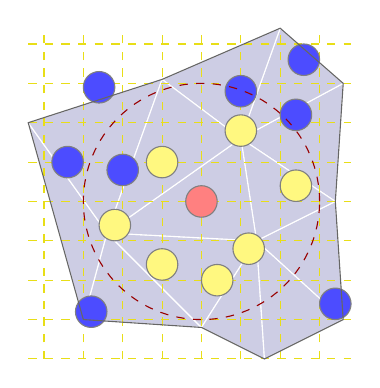
\begin{tikzpicture}
		%---Interno---
	%1 - (-1.2, -0.4)
	\draw[white, fill=blue!30!gray!30!white] (-1.5, -1.5) -- (0,-1.6) -- (-1.2, -0.4) -- cycle;
	\draw[white, fill=blue!30!gray!30!white] (-2.2, 1) -- (-1.5,-1.5) -- (-1.2, -0.4) -- cycle;
	\draw[white, fill=blue!30!gray!30!white] (-2.2, 1) -- (-0.5, 1.55) -- (-1.2, -0.4) -- cycle;
	%2 - (0.7, -0.5)
	\draw[white, fill=blue!30!gray!30!white] (-1.2, -0.4) -- (0,-1.6) -- (0.7, -0.5) -- cycle;
	\draw[white, fill=blue!30!gray!30!white] (0.8,-2) -- (0,-1.6) -- (0.7, -0.5) -- cycle;
	\draw[white, fill=blue!30!gray!30!white] (1.8,-1.5) -- (0.8,-2) -- (0.7, -0.5) -- cycle;
	\draw[white, fill=blue!30!gray!30!white] (1.8,-1.5) -- (1.7,0) -- (0.7, -0.5) -- cycle;
	%3 - (0.5,0.8)
	\draw[white, fill=blue!30!gray!30!white] (1.7,0) -- (1.8,1.5) -- (0.5, 0.8) -- cycle;
	\draw[white, fill=blue!30!gray!30!white] (1.7,0) -- (0.7, -0.5) -- (0.5, 0.8) -- cycle;
	\draw[white, fill=blue!30!gray!30!white] (1,2.2) -- (1.8,1.5) -- (0.5, 0.8) -- cycle;
	\draw[white, fill=blue!30!gray!30!white] (-0.5,1.55) -- (1,2.2) -- (0.5, 0.8) -- cycle;
	\draw[white, fill=blue!30!gray!30!white] (-1.2,-0.4) -- (0.7,-0.5) -- (0.5, 0.8) -- cycle;
	\draw[white, fill=blue!30!gray!30!white] (-1.2,-0.4) -- (-0.5,1.55) -- (0.5, 0.8) -- cycle;
	
	%malla
	\draw[step=0.5, dashed, yellow!90!black] (-2.2, -2) grid (1.9,2.2);
	
	%Partículas
	\draw[black!50, fill=red!50] (0,0) circle (2mm);
	\draw[black!50, fill=yellow!50] (0.6,-0.6) circle (2mm);
	\draw[black!50, fill=yellow!50] (-1.1,-0.3) circle (2mm);
	\draw[black!50, fill=yellow!50] (0.5,0.9) circle (2mm);
	\draw[black!50, fill=yellow!50] (-0.5,0.5) circle (2mm);
	\draw[black!50, fill=yellow!50] (1.2,0.2) circle (2mm);
	\draw[black!50, fill=yellow!50] (-0.5,-0.8) circle (2mm);
	\draw[black!50, fill=yellow!50] (0.2,-1) circle (2mm);
	
	\draw[black!50, fill=blue!70] (1.7,-1.3) circle (2mm);
	\draw[black!50, fill=blue!70] (-1.4,-1.4) circle (2mm);
	\draw[black!50, fill=blue!70] (-1,0.4) circle (2mm);
	\draw[black!50, fill=blue!70] (-1.7, 0.5) circle (2mm);
	\draw[black!50, fill=blue!70] (-1.3,1.45) circle (2mm);
	\draw[black!50, fill=blue!70] (1.2, 1.1) circle (2mm);
	\draw[black!50, fill=blue!70] (0.5,1.4) circle (2mm);
	\draw[black!50, fill=blue!70] (1.3,1.8) circle (2mm);
	
	%Carcasa
	\draw[black!60] (-2.2, 1) -- (-0.5, 1.55) -- (1, 2.2) -- (1.8, 1.5) -- (1.7, 0) -- (1.8, -1.5) -- (0.8, -2) -- (0, -1.6) -- (-1.5, -1.5) -- cycle;
	 
	 %Círculo rojo
	\draw[red!60!black, dashed] (0,0) circle (1.5 cm);
		\end{tikzpicture}
		\end{adjustbox}
		\caption{B\'usqueda de part\'iculas vecinas y c\'alculo de la fracci\'on de vac\'io de una part\'icula dada.}
	\end{subfigure}
	\hfill
	\begin{subfigure}[b]{0.3\textwidth}
		\centering
		\begin{adjustbox}{max width = \textwidth}
		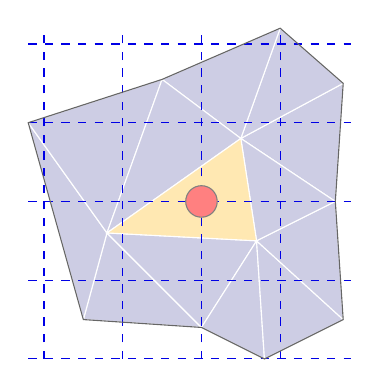
\begin{tikzpicture}
		%---Interno---
	%1 - (-1.2, -0.4)
	\draw[white, fill=blue!30!gray!30!white] (-1.5, -1.5) -- (0,-1.6) -- (-1.2, -0.4) -- cycle;
	\draw[white, fill=blue!30!gray!30!white] (-2.2, 1) -- (-1.5,-1.5) -- (-1.2, -0.4) -- cycle;
	\draw[white, fill=blue!30!gray!30!white] (-2.2, 1) -- (-0.5, 1.55) -- (-1.2, -0.4) -- cycle;
	%2 - (0.7, -0.5)
	\draw[white, fill=blue!30!gray!30!white] (-1.2, -0.4) -- (0,-1.6) -- (0.7, -0.5) -- cycle;
	\draw[white, fill=blue!30!gray!30!white] (0.8,-2) -- (0,-1.6) -- (0.7, -0.5) -- cycle;
	\draw[white, fill=blue!30!gray!30!white] (1.8,-1.5) -- (0.8,-2) -- (0.7, -0.5) -- cycle;
	\draw[white, fill=blue!30!gray!30!white] (1.8,-1.5) -- (1.7,0) -- (0.7, -0.5) -- cycle;
	%3 - (0.5,0.8)
	\draw[white, fill=blue!30!gray!30!white] (1.7,0) -- (1.8,1.5) -- (0.5, 0.8) -- cycle;
	\draw[white, fill=blue!30!gray!30!white] (1.7,0) -- (0.7, -0.5) -- (0.5, 0.8) -- cycle;
	\draw[white, fill=blue!30!gray!30!white] (1,2.2) -- (1.8,1.5) -- (0.5, 0.8) -- cycle;
	\draw[white, fill=blue!30!gray!30!white] (-0.5,1.55) -- (1,2.2) -- (0.5, 0.8) -- cycle;
	\draw[white, fill=blue!30!gray!30!white] (-1.2,-0.4) -- (-0.5,1.55) -- (0.5, 0.8) -- cycle;
	\draw[white, fill=red!30!yellow!30!white] (-1.2,-0.4) -- (0.7,-0.5) -- (0.5, 0.8) -- cycle;
	
	%malla
	\draw[step=1, dashed, blue!90!black] (-2.2, -2) grid (1.9,2.2);
	
	%Partículas
	\draw[black!50, fill=red!50] (0,0) circle (2mm);
	
	%Carcasa
	\draw[black!60] (-2.2, 1) -- (-0.5, 1.55) -- (1, 2.2) -- (1.8, 1.5) -- (1.7, 0) -- (1.8, -1.5) -- (0.8, -2) -- (0, -1.6) -- (-1.5, -1.5) -- cycle;
	 
		\end{tikzpicture}
		\end{adjustbox}
	\caption{Mapeo de una part\'icula dada dentro del fluido para interpolar sus propiedades en ese punto.}
	\end{subfigure}
	\hfill
	\begin{subfigure}[b]{0.3\textwidth}
		\centering
		\begin{adjustbox}{max width = \textwidth}
		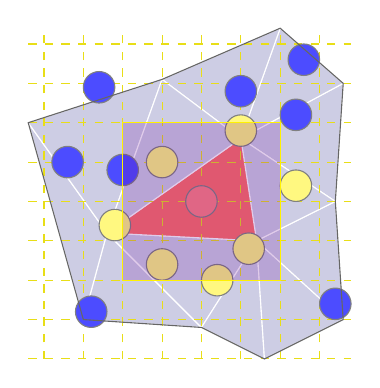
\begin{tikzpicture}
		%---Interno---
	%1 - (-1.2, -0.4)
	\draw[white, fill=blue!30!gray!30!white] (-1.5, -1.5) -- (0,-1.6) -- (-1.2, -0.4) -- cycle;
	\draw[white, fill=blue!30!gray!30!white] (-2.2, 1) -- (-1.5,-1.5) -- (-1.2, -0.4) -- cycle;
	\draw[white, fill=blue!30!gray!30!white] (-2.2, 1) -- (-0.5, 1.55) -- (-1.2, -0.4) -- cycle;
	%2 - (0.7, -0.5)
	\draw[white, fill=blue!30!gray!30!white] (-1.2, -0.4) -- (0,-1.6) -- (0.7, -0.5) -- cycle;
	\draw[white, fill=blue!30!gray!30!white] (0.8,-2) -- (0,-1.6) -- (0.7, -0.5) -- cycle;
	\draw[white, fill=blue!30!gray!30!white] (1.8,-1.5) -- (0.8,-2) -- (0.7, -0.5) -- cycle;
	\draw[white, fill=blue!30!gray!30!white] (1.8,-1.5) -- (1.7,0) -- (0.7, -0.5) -- cycle;
	%3 - (0.5,0.8)
	\draw[white, fill=blue!30!gray!30!white] (1.7,0) -- (1.8,1.5) -- (0.5, 0.8) -- cycle;
	\draw[white, fill=blue!30!gray!30!white] (1.7,0) -- (0.7, -0.5) -- (0.5, 0.8) -- cycle;
	\draw[white, fill=blue!30!gray!30!white] (1,2.2) -- (1.8,1.5) -- (0.5, 0.8) -- cycle;
	\draw[white, fill=blue!30!gray!30!white] (-0.5,1.55) -- (1,2.2) -- (0.5, 0.8) -- cycle;
	\draw[white, fill=red!95!yellow!60!white] (-1.2,-0.4) -- (0.7,-0.5) -- (0.5, 0.8) -- cycle;
	\draw[white, fill=blue!30!gray!30!white] (-1.2,-0.4) -- (-0.5,1.55) -- (0.5, 0.8) -- cycle;
	
	%malla
	\draw[step=0.5, dashed, yellow!90!black] (-2.2, -2) grid (1.9,2.2);
	
	%Partículas
	\draw[black!50, fill=red!50] (0,0) circle (2mm);
	\draw[black!50, fill=yellow!50] (0.6,-0.6) circle (2mm);
	\draw[black!50, fill=yellow!50] (-1.1,-0.3) circle (2mm);
	\draw[black!50, fill=yellow!50] (0.5,0.9) circle (2mm);
	\draw[black!50, fill=yellow!50] (-0.5,0.5) circle (2mm);
	\draw[black!50, fill=yellow!50] (1.2,0.2) circle (2mm);
	\draw[black!50, fill=yellow!50] (-0.5,-0.8) circle (2mm);
	\draw[black!50, fill=yellow!50] (0.2,-1) circle (2mm);
	
	\draw[black!50, fill=blue!70] (1.7,-1.3) circle (2mm);
	\draw[black!50, fill=blue!70] (-1.4,-1.4) circle (2mm);
	\draw[black!50, fill=blue!70] (-1,0.4) circle (2mm);
	\draw[black!50, fill=blue!70] (-1.7, 0.5) circle (2mm);
	\draw[black!50, fill=blue!70] (-1.3,1.45) circle (2mm);
	\draw[black!50, fill=blue!70] (1.2, 1.1) circle (2mm);
	\draw[black!50, fill=blue!70] (0.5,1.4) circle (2mm);
	\draw[black!50, fill=blue!70] (1.3,1.8) circle (2mm);
	
	%Carcasa
	\draw[black!60] (-2.2, 1) -- (-0.5, 1.55) -- (1, 2.2) -- (1.8, 1.5) -- (1.7, 0) -- (1.8, -1.5) -- (0.8, -2) -- (0, -1.6) -- (-1.5, -1.5) -- cycle;
	
	\draw[yellow, fill=red!40!blue, fill opacity=0.2] (-1,-1) rectangle (1,1);
		\end{tikzpicture}
		\end{adjustbox}
	\caption{Mapeo del elemento de malla CFD para el c\'alculo de t\'erminos fuente en el elemento de inter\'es.}
	\end{subfigure}
	\caption{Esquema de la aproximaci\'on por malla dual para la b\'usqueda de part\'iculas vecinas en un fluido.}
	\label{particle}
\end{figure}

\noindent
\justify

Los pasos clave con los que se basan las mallas de b\'usqueda son: detecci\'on de colisi\'on de part\'iculas (descrito en la secci\'on \ref{detect}), geometr\'ia de los elementos de malla CFD (detallado en la secci\'on \ref{CFD2D}) y el c\'alculo de fuerzas de fluido, entre otras.

\noindent
\justify

Para el c\'alculo de las fuerzas ejercidas por el fluido, se requiere conocer las propiedades del fluido en la posici\'on de la part\'icula; incluyendo el gradiente de presi\'on, la velocidad del flujo y el gradiente de velocidades (para fluidos gaseosos). Normalmente, las propiedades del fluido se `almacenan' en el centroide de los elementos de malla durante c\'alculos mediante FVM, como se muestra en la Ecuaci\'on \ref{properties}.

\begin{equation}
\phi _p = \phi _{el} + \nabla \phi _{el} \cdot r_{pc}
\label{properties}
\end{equation}

\noindent
\justify

D\'onde: $\phi _p$ y $\phi _{el}$ son las propiedades del fluido en la posici\'on de la part\'icula y el centroide del elemento, respectivamente; y $r_{pc}$ es el vector distancia que va desde el centro del elemento hasta la posici\'on de la part\'icula. 